\documentclass[../main.tex]{subfiles}
\begin{document}\label{chap2}

Chương \ref{chap1} đã đề cập đến hai công nghệ trong truyền thông không dây là bảo mật lớp vật lý và mạng vô tuyến nhận thức. Các công nghệ này sẽ được trình bày kỹ hơn trong chương này. Mở đầu chương là giới thiệu tổng quan về bảo mật lớp vật lý và các kỹ thuật giúp tăng cường sự an toàn. Sau đó, mạng vô tuyến nhận thức được đề cập cùng với các vấn đề liên quan, đặc biệt là vấn đề an toàn bảo mật. Hai nền tảng để mô hình hóa bài toán thiết kế nêu lên trong chương trước được trình bày ở phần cuối chương, đó là các độ đo hiệu năng an toàn sử dụng để đánh giá và mô hình toán học của lý thuyết tối ưu.

\section{An toàn bảo mật lớp vật lý}

An toàn bảo mật thường được tiếp cận từ khái niệm an toàn tuyệt đối (perfect secrecy) của Shannon \cite{shannon}, theo đó, hệ thống sử dụng một chiến lược mã hóa với khóa chia sẻ bí mật và đảm bảo bản mã không mang bất kỳ thông tin nào của thông điệp cần gửi. Mức độ an toàn này yêu cầu độ dài của khóa không ít hơn độ dài của thông điệp cần gửi, trong khi khóa là không dùng lại và cần được chia sẻ bí mật. Bài toán truyền tin bảo mật chuyển thành bài toán trao đổi khóa với độ phức tạp tương đương. Mặt khác, phạm vi của hướng tiếp cận trên giới hạn bởi giả thiết kênh truyền không nhiễu, xem xét trường hợp tệ nhất khi mà kẻ tấn công có thể thu được chính xác bản mã. Song trong thực tế, nhiễu là một thành phần không thể thiếu trong hầu hết các kênh truyền vật lý.

Ở hướng khác, Wyner \cite{wyner} giới thiệu mô hình kênh nghe lén (wiretap channel model), đánh giá ảnh hưởng của nhiễu trong truyền tin an toàn. Mô hình này đã đặt nền móng cho một hướng nghiên cứu gọi là bảo mật lớp vật lý. Mô hình của Wyner coi nhiễu như một đại lượng ngẫu nhiên giúp tăng khác biệt lợi thế giữa kênh truyền tới người dùng hợp pháp (gọi là kênh truyền chính - main channel) và kênh truyền tới kẻ tấn công (gọi là kênh truyền nghe lén - wiretap channel), cũng giống như lý thuyết của Shannon sử dụng khóa bí mật như một lợi thế về tính toán. Trong truyền thông không dây, cùng với nhiễu kênh truyền, các nghiên cứu sau này \cite{liang2008secure,barros2006secrecy,mukherjee2013fading,liang2013broadcast,tang2014secrecy,lin2015fast,lei2015physical} cũng cho thấy các đặc tính kênh truyền suy hao như đa đường (multipath) hay hiệu ứng bóng râm (shadow), mặc dù vốn có nhiều ảnh hưởng tiêu cực đến truyền tin tin cậy (chất lượng khôi phục tín hiệu tại người dùng hợp pháp), lại đóng góp rất nhiều trong việc tăng lợi thế này.

Khi các đặc tính kênh truyền không đủ để gia tăng đáng kể lợi thế giữa kênh truyền chính và kênh truyền nghe lén, một giải pháp được sử dụng là chèn nhiễu nhân tạo (artificial noise - AN) nhằm làm suy giảm chất lượng giải mã tín hiệu nhận tại bên nghe lén \cite{goel2008guaranteeing}. Nhiễu nhân tạo thường được triển khai trên các bộ hỗ trợ (helpers) hoặc sử dụng thêm các ăng-ten với kỹ thuật định hướng chùm tia \cite{zhou2011,cumanan2017secure,dong2009improving}. Ngoài ra, định hướng chùm tia hay hợp tác với các bộ hỗ trợ cũng có thể nhằm mục đích tăng cường chất lượng tín hiệu tại người dùng hợp pháp \cite{quach2017secrecy,dong2009improving}. Tuy nhiên các hướng tiếp cận này có một số hạn chế. Dưới góc nhìn thiết kế hệ thống, sinh nhiễu không mang thông tin như nhiễu nhân tạo là một giải pháp sử dụng năng lượng không hiệu quả, đồng thời làm giảm thông lượng mạng. Cùng với đó, kỹ thuật định hướng chùm tia cũng làm tăng độ phức tạp triển khai cho hệ thống \cite{sibomana2014impact} và việc sử dụng các bộ hỗ trợ cũng yêu cầu sự đồng bộ và tin tưởng \cite{yadav2021comprehensive}.

Mặt khác, kết quả từ \cite{tang2011interference} cho thấy can nhiễu từ một nguồn phát độc lập cũng giúp tăng hiệu quả an toàn ngay cả khi chất lượng của kênh truyền chính tệ hơn chất lượng trên kênh truyền nghe lén. Các kết quả nghiên cứu trong \cite{kalantari2015joint,xie2015secure,li2016} với các mô hình mạng đa người dùng đồng thời truyền tin cũng củng cố cho kết quả trên. Như vậy, so với kỹ thuật định hướng chùm kia và sự giúp đỡ từ các bộ hỗ trợ, hợp tác với các người dùng khác là một giải pháp đơn giản, tiết kiệm mà hiệu quả cho việc cải thiện mức độ an toàn.

\section{Mạng vô tuyến nhận thức và an toàn bảo mật}

Những năm gần đây, nhu cầu sử dụng phổ tần số ngày càng gia tăng với sự phát triển của các ứng dụng và dịch vụ trên nền tảng mạng không dây. Để tránh vấn đề can nhiễu, mỗi phần trong tài nguyên tần số chỉ cấp cho một hoặc một số người dùng, và chỉ những người dùng này có quyền khai thác phổ được cấp phát. Chính sách cấp phát tần số này được gọi là chính sách truy cập phổ cố định (fixed spectrum access - FSA). Thế nhưng, phần lớn dải tần số được cấp phát này lại chưa được khai thác hiệu quả \cite{liang2011}. Mạng vô tuyến nhận thức với chính sách truy cập phổ động (dynamic spectrum access - DSA) được đề xuất như một giải pháp cho vấn đề chưa tận dụng hiệu quả tài nguyên tần số. Mô hình này có hai kiểu người dùng chia sẻ truyền tin trên cùng một dải tần số là bên sơ cấp (primary user - PU) và bên thứ cấp (secondary user - SU). PU là những bên được cấp phép và có quyền ưu tiên hơn khi sử dụng dải tần số, còn SU là những bên mong muốn được sử dụng phần tài nguyên tần số được cấp phép đó.

Có hai chiến lược mà SU có thể triển khai để sử dụng dải tần số được cấp phép là truy cập phổ cơ hội (opportunistic spectrum access - OSA) và truy cập phổ đồng thời (concurrent spectrum access - CSA). Trong OSA, SU thực hiện cảm nhận phổ (spectrum sensing) để phát hiện phần phổ chưa được sử dụng (spectrum hole) và tự điều chỉnh các tham số truyền để tham gia. Tuy nhiên, khi chất lượng của pha cảm nhận phổ không tốt, SU vẫn có thể gây nhiễu lên bên nhận của PU \cite{sibomana2014impact}. Ở chiến lược CSA, SU có thể truyền đồng thời cùng với PU miễn là SU điều chỉnh công suất phát để can nhiễu gây cho bên nhận của PU nằm dưới một ngưỡng cho trước. Với chiến lược này, bằng việc thiết kế công suất phát hợp lý, hiệu quả sử dụng phổ có thể gia tăng đáng kể.

Khi xem xét vấn đề an toàn bảo mật, các nghiên cứu \cite{attar2012,salahdine2020security} đã khảo sát chi tiết các kỹ thuật tấn công và phòng vệ trong CRN. Các tấn công vào CRN bao gồm các tấn công truyền thống như chèn nhiễu (jamming) hay nghe lén (eavesdropping) và các tấn công nhằm vào CRN như cạnh tranh người dùng sơ cấp (PU emulation - PUE) hay giả mạo dữ liệu cảm biến phổ (spectrum sensing data falsification - SSDF). Đồ án này tập trung nghiên cứu về tấn công nghe lén trong CRN, ở đó kẻ tấn công đe dọa đến tính riêng tư của dữ liệu được truyền trong mạng bằng việc lợi dụng tính mở của môi trường truyền dẫn không dây.

\section{Thông tin kênh truyền trong an toàn bảo mật}

Trong truyền thông không dây, thông tin kênh truyền (channel state information - CSI) phản ánh tri thức mà các bên thu nhận có được về các đặc tính của kênh truyền như cách thức lan truyền tín hiệu hay các hiệu ứng suy hao. CSI tại các bên có thể đạt được thông qua quá trình ước lượng kênh với hai pha: (i) bên phát gửi tín hiệu huấn luyện và (ii) bên nhận phản hồi lại CSI, thường trên một liên kết riêng. Trong đó, CSI tại bên nhận (CSIR), hỗ trợ trong việc giải mã thông điệp, thường được giả thiết là hoàn hảo, chính xác (mặc dù thực tế vẫn có sai số ước lượng), trong khi CSI tại bên phát (CSIT) có thể giả thiết ở nhiều mức độ khác nhau, thông qua chất lượng của pha phản hồi \cite{hyadi2016overview}.

CSIT đóng vai trò rất quan trọng, tri thức về kênh truyền càng chính xác, bên phát có thể lựa chọn chiến lược mã hóa và xử lý tín hiệu càng tối ưu cho các độ đo hiệu năng. Với truyền tin an toàn, chiến lược truyền phụ thuộc cả vào chất lượng CSIT trên kênh truyền chính và CSIT trên kênh truyền nghe lén. Tuy nhiên, CSIT đầy đủ thường không đạt được trong thực tế, đặc biệt là CSIT về kênh truyền nghe lén vì kẻ nghe lén có thể không tương tác với bên ngoài (nghe lén thụ động), và như vậy bên phát không có phản hồi CSI về kênh truyền này \cite{he2013wireless}.

Các nghiên cứu sâu rộng về ảnh hưởng của các mức CSIT khác nhau cũng cho thấy một số kỹ thuật giúp tăng cường mức độ an toàn ngay cả khi thông tin về kênh truyền tại bên phát không đầy đủ. Trong trường hợp bên phát chỉ có một ăng-ten, các nghiên cứu \cite{he2013secure,zhou2011,gopala2008secrecy,rezki2011ergodic,he2016secrecy} đề xuất chiến lược truyền "on-off": bên phát quyết định truyền hoặc hoãn truyền tin dựa trên tri thức có từ bên nhận. Phản hồi từ bên nhận có thể là kết quả ước lượng CSI \cite{gopala2008secrecy,he2013secure,zhou2011,rezki2011ergodic} hoặc có thể chỉ cần một bit \cite{he2016secrecy,zhou2011}. Trong trường hợp bên phát có nhiều ăng-ten, kỹ thuật định hướng chùm tia kết hợp với nhiễu nhân tạo được sử dụng rộng rãi \cite{goel2008guaranteeing,zhang2013design}, ngoài ra, có thể triển khai "on-off" mức ăng-ten trong chiến lược lựa chọn ăng-ten phát (transmit antenna selection - TAS) \cite{alves2016enhanced}. Như vậy, ngay cả khi chỉ có được thông tin kênh truyền rất ít, bên phát vẫn có cơ hội lựa chọn chiến lược truyền tin an toàn.

\section{Các độ đo hiệu năng an toàn}

Các độ đo đánh giá mức độ an toàn trong PLS được phát triển từ lý thuyết thông tin với mô hình truyền tin đơn giản gồm ba đối tượng. Bên phát (Alice) cần truyền một thông điệp $M$ tới người dùng hợp pháp (Bob). Để giữ bí mật $M$ với kẻ nghe lén (Eve), Alice sử dụng một bộ mã hóa ngẫu nhiên (stochastic encoder \cite{wyner}) mã hóa $M$ thành $X^n$ với $n$ là số lượt truy cập kênh (channel uses). Dưới tác động của các kênh truyền, Bob và Eve tương ứng thu được phiên bản $Y^n$ và $Z^n$ của $X^n$. Một bộ mã hóa xác định có hai tham số quan trọng là tốc độ truyền từ mã (codewords transmission rate) $R_b = \frac{H\left(X^n\right)}{n}$ và tốc độ truyền tin (transmission rate/confidential information rate) $R_s = \frac{H\left(M\right)}{n}$, trong đó ký hiệu $H(X)$ là lượng tin riêng (entropy) của $X$. Ngoài ra, một đại lượng cũng thường sử dụng trong lý thuyết thông tin là tốc độ không rõ ràng của kẻ nghe lén (eavesdropper's equivocation rate) $R_e = \frac{H\left(M | Z^n\right)}{n}$, với ký hiệu $H(X|Y)$ là lượng tin riêng của $X$ với điều kiện $Y$. Đại lượng này phản ánh tốc độ tin trung bình mà kẻ nghe lén không biết về thông điệp truyền. Các độ đo mức độ an toàn dưới đây có liên quan mật thiết tới các đại lượng này.

\subsection{Dung lượng an toàn và tốc độ an toàn}

Trong việc lựa chọn độ đo đánh giá mức độ an toàn, chất lượng CSIT cũng đóng vai trò quan trọng. Với CSIT hoàn hảo cho cả kênh truyền chính và kênh truyền nghe lén, dung lượng an toàn (secrecy capacity - SC) $C_s$ \cite{barros2006secrecy} thường được sử dụng để phân tích hiệu quả an toàn của hệ thống:
\begin{equation}\label{metric:cs}
    C_s = \max\left(C_B - C_E, 0\right),
\end{equation}
trong đó $C_B$ và $C_E$ tương ứng là dung lượng (tức thời) của kênh truyền chính và kênh truyền nghe lén, được tính dựa trên chất lượng tín hiệu nhận, phản ánh thông qua tỷ số tín hiệu trên nhiễu (signal-to-noise ratio - SNR). Dung lượng an toàn xác định giới hạn trên cho tốc độ truyền tin an toàn $R_s$ (secrecy rate) của hệ thống, là tốc độ truyền tin lớn nhất đạt được vẫn đảm bảo kẻ nghe lén không thể giải mã thông điệp.

Với CSIT không hoàn hảo, dung lượng an toàn ergodic \cite{gopala2008secrecy,rezki2011ergodic} và xác suất mất an toàn \cite{parada2005secrecy,barros2006secrecy} thường được sử dụng. Song, dung lượng an toàn ergodic chỉ phù hợp với các hệ thống chấp nhận độ trễ cao do tín hiệu truyền cần khoảng thời gian để trải nghiệm đủ thể hiện của kênh \cite{he2013wireless}. Do đó, đồ án chỉ giới thiệu các độ đo dựa trên xác suất mất an toàn.

\subsection{Xác suất mất an toàn}

Xác suất mất an toàn (secrecy outage probability - SOP) xác định xác suất hệ thống không đạt được một tốc độ truyền tin an toàn $R_s$ cho trước:
\begin{equation}\label{sop}
    \text{SOP} = \mathbb{P}\left(C_s < R_s\right).
\end{equation}
Tham số $R_s$ được lựa chọn dựa trên ước lượng của Alice về khả năng giải mã tin của Eve: khi $C_s < R_s$ hay $C_E > C_B - R_s$ thì Eve có thể giải mã tin với tốc độ cao hơn mong đợi, tức là thông tin bị rò rỉ \cite{barros2006secrecy}.

\subsection{Công thức khác cho xác suất mất an toàn}

Dựa trên công thức \eqref{sop}, có thể thấy SOP đánh giá hai sự kiện gây mất an toàn là (i) thông tin bị rò rỉ tới Eve hoặc (ii) Bob không thể giải mã chính xác thông điệp. Tức là, SOP đánh giá hệ thống ở cả tính tin cậy và an toàn. Nhằm tách biệt hai mục tiêu này, tác giả Zhou và cộng sự \cite{zhou2011} đề xuất một công thức khác cho SOP (gọi là ASOP - alternative secrecy outage probability):
\begin{equation}\label{asop}
    \text{ASOP} = \mathbb{P}\left(C_E > R_b - R_s \mid \text{message transmission}\right).
\end{equation}
Khi thêm điều kiện cho công thức, việc xác định chiến lược truyền phù hợp có thể giúp gia tăng hiệu quả an toàn (giảm SOP) do chỉ đánh giá hiệu năng tại những phiên truyền thực tế giữa Alice và Bob. Ví dụ nếu Alice có thể xác định khả năng giải mã của Bob thì Alice có thể tạm dừng truyền tin trong một khoảng thời gian.

\subsection{Các độ đo dựa trên mức độ không rõ ràng}

Bằng việc chỉ ra các hạn chế của SOP như (i) không cho thấy khả năng giải mã của kẻ nghe lén và (ii) không cho thấy lượng tin bị lộ, tác giả He và cộng sự \cite{he2016secrecy} đề xuất ba độ đo hiệu năng cho phép đánh giá \textit{mức độ an toàn một phần} (partial secrecy), dựa trên mức độ không rõ ràng của kẻ nghe lén $\Delta = H(M \mid Z^n)/H(M)$. Đối với kênh truyền suy hao, mức độ không rõ ràng tối đa có thể đạt được là:
\begin{equation}\label{delta}
    \Delta= 
\begin{cases}
    1,& \text{nếu} \quad C_E\leq C_B - R_s\\
    \left(C_B - C_E\right)/R_s,& \text{nếu} \quad C_B - R_s < C_E < C_B\\
    0              ,& \text{nếu} \quad C_B \leq C_E.
\end{cases}
\end{equation}

Từ đây, ba độ đo mới được đề xuất, dựa trên đánh giá phân bố của $\Delta$.

1. Xác suất mất an toàn tổng quát (generalized SOP - GSOP)

Xác suất mất an toàn tổng quát được biểu diễn theo phân phối tích lũy của $\Delta$:
\begin{equation}\label{gsop}
    \text{GSOP} = \mathbb{P}(\Delta < \theta),
\end{equation}
trong đó $\theta \in \left(0, 1\right]$ là hằng số chọn trước, phản ánh tỷ lệ lượng tin yêu cầu tối thiểu mà Eve không biết về thông điệp truyền $M$, nói cách khác, $\left(1 - \theta\right)$ phản ánh tỷ lệ lượng tin bị tiết lộ tối đa chấp nhận được của hệ thống \cite{he2016secrecy}. Khi $\theta = 1$, hệ thống yêu cầu mức an toàn cao nhất, tức là không để lộ bất kỳ lượng tin nào tới Eve, tương đương với SOP.

2. Tỷ lệ không rõ ràng trung bình (average fractional equivocation)

Giá trị trung bình của $\Delta$ có thể dùng làm tiệm cận dưới cho xác suất giải mã sai tại bên nghe lén \cite{he2016secrecy}:
\begin{equation}\label{delta-expectation}
    \bar{\Delta} = \mathbb{E}\left\{\Delta\right\}.
\end{equation}

3.  Tốc độ lộ thông tin trung bình (average information leakage rate - AILR)

Khác với xác suất mất an toàn, tốc độ lộ thông tin giúp phân tích định lượng hiệu năng an toàn của hệ thống. Các thiết kế truyền tin an toàn có thể đạt được xác suất mất an toàn như nhau nhưng lại khác nhau về tốc độ lộ thông tin \cite{he2016secrecy}. Tốc độ lộ thông tin trung bình có thể được xác định dựa trên mức độ không rõ ràng của kẻ nghe lén $\Delta$, vì $(1 - \Delta)$ phản ánh lượng thông tin mà Eve có được về thông điệp truyền. Tóm lại, tốc độ thông tin bị lộ trung bình có công thức:
\begin{equation}\label{ailr}
    R_L = \mathbb{E}\left\{\frac{I\left(M, Z^n\right)}{n}\right\} = \mathbb{E}\left\{(1-\Delta)R_s\right\}.
\end{equation}
Khi tốc độ truyền tin $R_s$ không đổi, công thức này có thể đưa về dạng đơn giản:
\begin{equation}\label{ailr-fixed}
    R_L = \left(1-\bar{\Delta}\right)R_s.
\end{equation}

\section{Tối ưu trong bài toán thiết kế}

Các nghiên cứu về an toàn bảo mật lớp vật lý thường tập trung vào hai khía cạnh: (i) phân tích hệ thống theo lý thuyết thông tin, với các nghiên cứu liên quan đến dung lượng an toàn và tốc độ an toàn, (ii) thiết kế hệ thống, với các nghiên cứu về xử lý tín hiệu, cấp phát tài nguyên và hợp tác. Với ý nghĩa thực tiễn, vấn đề thiết kế hệ thống an toàn bảo mật ngày càng được quan tâm nghiên cứu, trong đó lý thuyết tối ưu thường được sử dụng vì ý tưởng tìm kiếm trạng thái tốt nhất giúp hệ thống đạt được hiệu năng cao nhất.

\subsection{Bài toán tối ưu}

Bài toán tối ưu được mô tả dưới dạng tổng quát sau:
\begin{equation}\label{def:opt}
\begin{aligned}
\underset{\mathbf{x}}{\text{minimize}} \quad & f\left(\mathbf{x}\right) \\
\textrm{s.t} \quad & h_i\left(\mathbf{x}\right) \geq b_i, & i=1,2,\dots,p \\
\quad & g_j\left(\mathbf{x}\right) = c_j, & j=1,2,\dots,q,\\
\end{aligned}
\end{equation}
trong đó $\mathbf{x}$ là một véc-tơ $n$-chiều, được gọi là biến quyết định hay biến tối ưu và $f: \mathbb{R}^n \rightarrow \mathbb{R}$ được gọi là hàm mục tiêu, hay hàm chi phí, mục tiêu của bài toán là giảm giá trị hàm mục tiêu này. Các điều kiện $h_i(x) \leq b_i$ và $g_j(x)=c_j$ tương ứng là các ràng buộc bất đẳng thức và ràng buộc đẳng thức của bài toán. Các ràng buộc này giới hạn một tập giá trị hợp lệ (feasible set) mà các biến quyết định có thể nhận, đồng thời cũng giới hạn tập giá trị mà hàm mục tiêu có thể đạt được (feasible objective set).

Giải quyết bài toán này là quá trình đi tìm một điểm thỏa mãn các điều kiện ràng buộc trong không gian các biến quyết định (decision space) mà giá trị của hàm mục tiêu ứng với điểm đó là nhỏ nhất trong tập các điểm hợp lệ. Điểm như vậy được gọi là nghiệm tối ưu toàn cục. Việc tìm kiếm nghiệm tối ưu toàn cục thường không dễ dàng với hầu hết các bài toán tối ưu, do việc này đòi hỏi việc kiểm tra trên toàn bộ tập các giá trị hợp lệ, ngoại trừ một số ít lớp bài toán có thể kiểm tra tính toàn cục của một nghiệm tìm được. Mặt khác, trong nhiều bài toán, việc tìm kiếm một giá trị tối ưu toàn cục là không cần thiết. Do đó, trong các vấn đề thiết kế thực tế, bài toán tối ưu thường hướng đến tìm kiếm lời giải nhanh và dễ dàng hơn khi chỉ tìm kiếm các nghiệm tối ưu cục bộ: trong số các điểm hợp lệ lân cận thì giá trị hàm mục tiêu tại nghiệm tối ưu cục bộ là nhỏ nhất.

\subsection{Các phương pháp giải quyết bài toán tối ưu một mục tiêu}

Với lịch sử phát triển lâu dài, các nghiên cứu về lý thuyết tối ưu đã giới thiệu rất đa dạng các phương pháp giải quyết cho nhiều lớp bài toán tối ưu \cite{10.5555/3351864}. Tuy nhiên, không có phương pháp nào hiệu quả với mọi bài toán. Các phương pháp thường đặt ra một số yêu cầu về bài toán cần giải quyết như tính chất lồi của hàm mục tiêu và tập giá trị hợp lệ \cite{boyd2004convex} hay chỉ phù hợp với bài toán có số lượng nhỏ các biến quyết định và các điều kiện ràng buộc. Do đó, quá trình lựa chọn phương pháp giải bài toán tối ưu không chỉ dựa trên mức độ hiệu quả và tốc độ thực thi của phương pháp mà cần cân nhắc cả về đặc điểm của bài toán cần giải quyết.

Các phương pháp giải quyết bài toán tối ưu thường triển khai theo các bước lặp: với một ước lượng ban đầu về nghiệm của bài toán tối ưu, trong hữu hạn các lần lặp, các phương pháp tìm cách sinh các giá trị cho biến quyết định nhằm làm cho hàm mục tiêu hội tụ về giá trị nhỏ nhất của nó. Các phương pháp khác nhau có chiến lược lựa chọn giá trị biến quyết định cho các vòng lặp khác nhau. Có rất nhiều phương pháp có tính ứng dụng cao đã khai thác hiệu quả tính khả vi của hàm mục tiêu trong việc tìm kiếm nghiệm tối ưu của bài toán. Cơ sở lý thuyết của ý tưởng này nằm ở tính chất: đạo hàm cấp một (đối với hàm một biến) hay gradient (đối với hàm nhiều biến) thể hiện tốc độ thay đổi giá trị của hàm số tại một điểm, đồng thời cũng xác định hướng biến thiên của hàm số tại điểm đó. Điều đó cho thấy, tại mỗi vòng lặp, thông tin về gradient (hay đạo hàm) có thể được dùng để định hướng tới nghiệm tối ưu của bài toán, giá trị của biến quyết định trong vòng lặp tiếp theo chỉ cần cập nhật dựa trên giá trị hiện tại cùng với hướng giảm xác định được của hàm mục tiêu. Các nghiên cứu sâu rộng dựa trên ý tưởng sử dụng gradient đã giới thiệu những kỹ thuật xử lý đặc biệt giúp cải thiện đáng kể tốc độ hội tụ của bài toán. Tuy nhiên, các phương pháp này đều có chung một hạn chế, nằm ở ý tưởng của phương pháp, đó là lời giải của bài toán phụ thuộc vào giá trị khởi tạo của biến quyết định. Với một thủ tục và một giá trị khởi tạo xác định, các phương pháp này thường chỉ lựa chọn các giá trị cho biến quyết định nằm trên một hoặc một số hướng tìm kiếm. Như vậy, rất khó để đảm bảo nghiệm tìm được là tối ưu toàn cục. 

Một hướng tiếp cận giúp vượt qua hạn chế của các phương pháp đề cập ở trên là sinh một tập hợp các giá trị các biến quyết định (thay vì chỉ một) trong mỗi vòng lặp. Các phương pháp này được gọi là các phương pháp dựa trên quần thể (population based methods), mỗi giá trị của biến quyết định được gọi là một cá thể (individual). Hầu hết ý tưởng của các phương pháp dựa trên quần thể đều lấy cảm hứng từ tự nhiên với hai nhóm giải thuật là giải thuật tiến hóa (evolution algorithms) và giải thuật dựa trên trí tuệ bầy đàn (swarm intelligence-based algorithms). Các giải thuật tiến hóa lấy cảm hứng từ quá trình chọn lọc tự nhiên và cơ chế lai tạo giữa các cá thể trong một quần thể sinh học. Cụ thể, trong mỗi thế hệ (mỗi vòng lặp), các bộ hai cá thể được lựa chọn để lai tạo ra các cá thể mới (crossover), cá thể mới này mang những đặc điểm của hai cá thể cha mẹ, ngoài ra có cả những đặc điểm đột biến (mutation). Thông qua quá trình chọn lọc tự nhiên, những cá thể mang đặc điểm có lợi (ứng với các biến quyết định làm cho hàm mục tiêu nhỏ) có khả năng sống sót cao hơn (được giữ lại trong các vòng lặp tiếp theo). Qua mỗi thế hệ, chất lượng của cả quần thể được cải thiện, tương ứng với đó là tập các biến quyết định có xu hướng hội tụ về nghiệm tối ưu của bài toán. Đối với các giải thuật dựa trên trí tuệ bầy đàn, ý tưởng được lấy cảm hứng từ hành vi và cách thức liên lạc giữa các cá thể trong quần thể động vật. Với trí tuệ bầy đàn, các cá thể có thể hành động độc lập và không cần kiểm soát tập trung, song với chung một mục tiêu, sự tương tác (cục bộ) giữa các cá thể có thể giúp cho cả quần thể hành động như một thể thống nhất, từ đó có thể giải quyết những bài toán phức tạp. Có thể thấy, các phương pháp dựa trên quần thể không chỉ giúp khám phá không gian biến quyết định để tăng khả năng tìm kiếm nghiệm toàn cục, mà còn khai thác thông tin từ các cá thể để giúp bài toán hội tụ tại nghiệm tốt nhất trong không gian tìm kiếm xác định được.

Các phương pháp dựa trên quần thể cho thấy tiềm năng trong việc giải quyết các bài toán tối ưu khó vì không đặt ra các giả thiết về bài toán cần giải quyết và cũng không dựa trên gradient, vốn không phải dễ dàng có được đối với nhiều hàm mục tiêu. Mặc dù nghiệm giải được của bài toán theo các phương pháp này không đảm bảo là tối ưu toàn cục nhưng trong hầu hết trường hợp, kết quả thu được là thỏa mãn mong muốn về nghiệm của người dùng. Đồ án này giới thiệu một giải thuật trong nhóm phương pháp này, giải thuật tiến hóa vi phân (differential evolution - DE), vì tính hiệu quả cũng như sự phù hợp đối với lớp bài toán tối ưu liên tục (không gian biến quyết định là liên tục). 

Tiến hóa vi phân DE là một giải thuật tiến hóa được giới thiệu lần đầu bởi Storn và Price \cite{storn1997differential}. Cũng giống như các giải thuật tiến hóa khác, DE duy trì một tập $NP$ cá thể, mỗi cá thể có $D$ thuộc tính (tương ứng với số chiều của không gian biến quyết định) và biến đổi chúng qua các thế hệ $G = 0, 1,\ldots, G_{max}$ với ba thao tác: lai tạo (crossover), đột biến (mutation) và chọn lọc (selection). Ký hiệu cá thể thứ $i$ trong thế hệ $G$ là $X_{i,G} = \left[x_{1,i,G}, x_{2,i,G},\ldots,x_{D,i,G}\right], i = 1,2,\ldots,NP$. Thế hệ $0$ là thế hệ khởi tạo của quần thể, các cá thể thường được sinh ngẫu nhiên với mục tiêu chúng có thể phân bố rộng khắp phạm vi tìm kiếm. Tại các thế hệ sau, các cá thể mới được tạo ra bằng cách lai giữa các cặp cá thể mục tiêu và cá thể đột biến. Điểm khác biệt quan trọng trong ý tưởng của DE so với các giải thuật tiến hóa khác là cách tạo ra cá thể đột biến: cá thể này được tạo dựa trên chính các cá thể trong quần thể hiện tại. Cụ thể, DE lựa chọn ngẫu nhiên ba cá thể khác nhau $X_{r_1^i}$, $X_{r_2^i}$ và $X_{r_3^i}$, trong đó hai cá thể bất kỳ dùng làm đại lượng đột biến cho cá thể còn lại: 
\begin{equation}
    V_{i,G} = X_{r_1^i,G} + F.\left(X_{r_2^i,G} - X_{r_3^i,G}\right),
\end{equation}
trong đó $V_{i,G}$ là cá thể đột biến và $F$ là biên độ đột biến (scaling factor/mutation constant), là tham số chọn trước trong thuật toán. Có thể thấy, DE khai thác thông tin từ chính phân bố của quần thể để quyết định mức độ đột biến: nếu các cá thể phân bố xa nhau thì lượng đột biến cũng lớn và khi chúng ở gần nhau (tức là bài toán dần hội tụ) thì chỉ cần ít sự đột biến. Điều này giúp các thế hệ đầu có thể khám phá không gian tìm kiếm mà vẫn đảm bảo lựa chọn nghiệm tốt nhất ở các thế hệ sau. Cá thể đột biến $V_{i,G}$ sau đó được lai tạo với cá thể mục tiêu $X_{i,G}$ bằng cách chọn ngẫu nhiên mỗi thuộc tính từ một trong hai cá thể này làm thuộc tính cho cá thể mới. Mức độ ngẫu nhiên này được phản ánh thông qua một tham số gọi là tốc độ lai tạo $CR$ (crossover rate), phản ánh xác suất một thuộc tính có thể bị đột biến trong cá thể lai tạo. Một trong những chiến lược lai tạo thường dùng trong DE là lai tạo đồng bộ (uniform crossover/binomial):
\begin{equation}
u_{j,i,G} = 
\begin{cases}
    v_{j,i,G},& \text{nếu} \quad rand \leq CR \ \text{hoặc}\ j = j_{rand} \\
    x_{j,i,G},& \text{trong trường hợp còn lại},
\end{cases}
\end{equation}
với $rand$ là một giá trị ngẫu nhiên (với phân bố đều) trên đoạn $\left[0;1\right]$ và $j_{rand}$ là một chỉ số chọn ngẫu nhiên trên đoạn $\left[1;D\right]$, giá trị này được thêm vào với mục đích đảm bảo luôn có ít nhất một thuộc tính của cá thể đột biến được kế thừa. Để đảm bảo chất lượng quần thể không tệ hơn qua các thế hệ, cá thể mới $U_{i,G}$ cần được so sánh với cá thể mục tiêu $X_{i,G}$, cá thể nào trội hơn (với nghĩa là giá trị tương ứng của hàm mục tiêu nhỏ hơn) sẽ được giữ lại cho thế hệ tiếp theo:
\begin{equation}
X_{i,G+1} = 
\begin{cases}
    U_{i,G},& \text{nếu} \quad f(U_{i,G}) \leq f(X_{i,G}) \\
    X_{i,G},& \text{trong trường hợp còn lại}.
\end{cases}
\end{equation}
Các quá trình đột biến, lai tạo và chọn lọc trên được lặp lại qua các thế hệ cho đến khi quần thể đạt đến trạng thái dừng. Trạng thái dừng có thể được xác định theo một số cách sau: (i) sau một số thế hệ xác định $G_{max}$, (ii) cá thể trội nhất của quần thể không đổi sau một chuỗi liên tiếp các thế hệ, hoặc (iii) đạt được một giá trị hàm mục tiêu mong muốn. Như vậy, có thể thấy, DE là một thuật giải không chỉ đơn giản, dễ triển khai, ít tham số cấu hình, phù hợp với nhiều bài toán, mà còn hiệu quả trong việc tìm kiếm nghiệm tối ưu toàn cục qua việc khám phá và khai thác không gian biến quyết định.

\subsection{Tối ưu đa mục tiêu}

Mô hình hóa bài toán thiết kế an toàn bảo mật với chỉ một hàm mục tiêu không phải lúc nào cũng dễ dàng, bởi cần cân nhắc giữa các độ đo hiệu năng (như tính tin cậy và tính an toàn) hoặc giữa lợi ích của các bên (trong hệ thống đa người dùng). Lúc này, xây dựng bài toán với chỉ một hàm mục tiêu cho thấy sự thiên vị ngay từ bước mô hình hóa bài toán. Với những vấn đề thiết kế này, lựa chọn phù hợp là mô hình hóa bài toán tối ưu với nhiều hàm mục tiêu, hay gọi là bài toán tối ưu đa mục tiêu (multiobjective optimization problem - MOOP):
\begin{equation}\label{def:moop}
\begin{aligned}
\underset{\mathbf{x}}{\text{minimize}} \quad & f_k\left(\mathbf{x}\right), \quad k=1,2,\dots,m \\
\textrm{s.t} \quad & h_i\left(\mathbf{x}\right) \geq b_i, \quad i=1,2,\dots,p \\
\quad & g_j\left(\mathbf{x}\right) = c_j, \quad j=1,2,\dots,q.\\
\end{aligned}
\end{equation}
Điểm khác biệt duy nhất của bài toán này so với bài toán tối ưu \eqref{def:opt} là số lượng các hàm mục tiêu, $m > 1$, tức là không gian giá trị các hàm mục tiêu (không gian mục tiêu - objective space) trở thành không gian đa chiều $\mathbb{R}^m$.

Khi chỉ có một hàm mục tiêu, các giá trị khác nhau của biến quyết định có thể dễ dàng được xếp hạng dựa trên giá trị của hàm mục tiêu tương ứng (lúc này chỉ là các số thực), từ đó có thể đánh giá một điểm hợp lệ có là "tối ưu" hay không. Tuy nhiên, khái niệm "tối ưu" này không thể áp dụng trực tiếp vào bài toán tối ưu đa mục tiêu, vì không gian mục tiêu là nhiều chiều, không phải lúc nào cũng so sánh được hai véc-tơ giá trị với nhau. Vì thế, khái niệm "tối ưu Pareto" thường được sử dụng để định nghĩa nghiệm của bài toán tối ưu đa mục tiêu: một biến quyết định hợp lệ được gọi là tối ưu Pareto nếu như tất cả các biến quyết định hợp lệ khác nếu giúp cải thiện giá trị một hàm mục tiêu thì phải làm ít nhất một hàm mục tiêu khác tệ hơn. Về mặt toán học, biến quyết định hợp lệ $\mathbf{x^*}$ được gọi là tối ưu Pareto nếu không tồn tại một biến quyết định hợp lệ $\mathbf{x}$ nào khác thỏa mãn đồng thời $f_k\left(\mathbf{x}\right) \leq f_k\left(\mathbf{x^*}\right), \forall\ k=1,2,\ldots,m$ và $\exists\ l: f_l\left(\mathbf{x}\right) < f_l\left(\mathbf{x^*}\right)$. Việc tìm kiếm nghiệm tối ưu Pareto thường thu được một tập kết quả, ảnh của tập nghiệm đó được gọi là biên Pareto (Pareto front).  Hình~\ref{fig:Pareto} biểu diễn biên Pareto trong không gian mục tiêu với hai hàm mục tiêu $f_1$ và $f_2$, trong đó đường cong kín mô tả tập giá trị có thể nhận của các hàm mục tiêu và phần biên được bôi đậm là biên Pareto. Có thể thấy, tập giá trị có thể nhận của các hàm mục tiêu có thể lồi (convex, tất cả các điểm nằm trên đoạn nối hai điểm bất kỳ trong tập hợp đều là phần tử của tập đó) hoặc không lồi (non-convex). Trong hình này, tập giá trị có thể nhận của các hàm mục tiêu là không lồi tại biên Pareto.

\begin{figure}
\centering
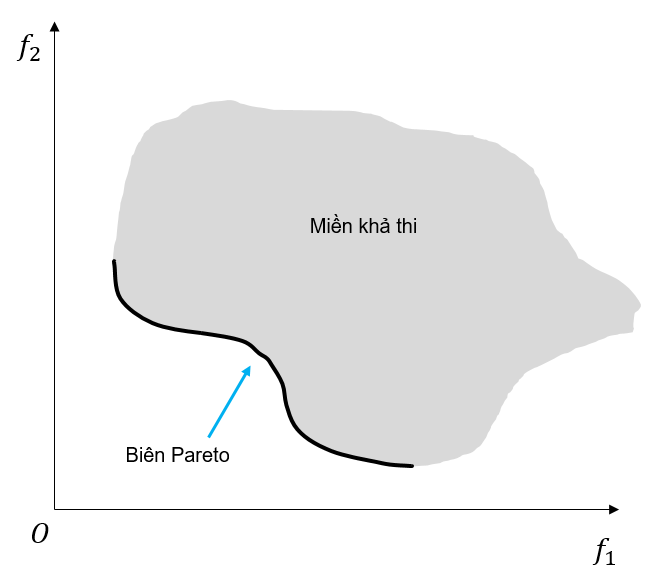
\includegraphics[width=0.8\linewidth]{pareto-front.png}
\caption{Biên Pareto}
\label{fig:Pareto}
\end{figure}

Định nghĩa bài toán thiết kế theo một mô hình khác cũng dẫn đến lời giải cho bài toán tối ưu cũng được xác định theo hướng khác. Khi có nhiều mục tiêu để tối ưu, các mục tiêu này có thể xung đột với nhau: giảm giá trị hàm mục tiêu này dẫn đến tăng giá trị cho hàm mục tiêu khác, và như vậy không có giá trị nào của biến quyết định làm cho mọi hàm mục tiêu cùng đạt đến giá trị nhỏ nhất có thể của nó. Lúc này, sự cân nhắc về mức độ ưu tiên giữa các mục tiêu trong quá trình thiết kế mô hình chuyển thành việc lựa chọn một nghiệm tối ưu phù hợp với mong muốn của người dùng. Việc lựa chọn này có thể được giải quyết với các bộ quyết định (decision makers). Các bộ quyết định, với khả năng so sánh giữa các lời giải khác nhau theo sự ưu tiên của người dùng, có thể lựa chọn một lời giải phù hợp nhất trong tập các lời giải tìm được. 

\subsection{Các phương pháp giải quyết bài toán tối ưu đa mục tiêu}

Về mặt toán học, việc tìm kiếm toàn bộ nghiệm tối ưu Pareto có thể coi như giải quyết xong bài toán tối ưu đa mục tiêu. Tuy nhiên, trong thực tế, số lượng các nghiệm này là rất lớn, trong khi, mục tiêu của việc giải bài toán này là lựa chọn một lời giải phù hợp nhất với mong muốn của người dùng. Như vậy, thay vì tìm kiếm toàn bộ nghiệm, các phương pháp giải chỉ cần đề xuất tới các bộ quyết định một hoặc một tập hữu hạn các lời giải tối ưu Pareto.

Các phương pháp giải bài toán tối ưu đa mục tiêu có thể nhóm thành ba nhóm \cite{collette2004multiobjective}. Thứ nhất là nhóm các phương pháp tiên nghiệm (priori methods), ở đó mong muốn của người dùng về kết quả được xác định trước khi tiến hành tìm kiếm lời giải. Như vậy, việc tìm kiếm chỉ cần trả về một nghiệm phản ánh tốt nhất mong muốn đã đặt ra. Tuy nhiên, không phải lúc nào cũng có thể biểu diễn chính xác mong muốn về kết quả, tức là rất khó xác định hướng tìm kiếm nghiệm ngay từ đầu. Nhóm thứ hai là các phương pháp lũy tiến (progressive methods). Các phương pháp này đòi hỏi các bộ quyết định tham gia trong suốt quá trình tìm kiếm lời giải, với vai trò đánh giá kết quả, giúp điều chỉnh hướng tìm kiếm nhằm đi đến nghiệm phù hợp nhất với mong muốn người dùng. Hạn chế lớn nhất của nhóm phương pháp này là việc đòi hỏi sự tham gia và phản hồi liên tục từ các bộ quyết định, cùng với đó, tốc độ phản hồi cũng ảnh hưởng đến thời gian thực thi của phương pháp. Thứ ba là nhóm các phương pháp hậu nghiệm (posteriori methods). Khác với các nhóm phương pháp trước, các phương pháp trong nhóm này thực hiện tìm kiếm và đề xuất một tập hữu hạn các lời giải để các bộ quyết định lựa chọn. Mặc dù không đòi hỏi phải biểu diễn mong muốn về kết quả hay sự phản hồi liên tục từ các bộ quyết định, ý tưởng sinh nhiều lời giải ở các phương pháp thuộc nhóm này lại khiến thời gian thực thi tăng lên đáng kể so với việc chỉ tìm kiếm một nghiệm. Bên cạnh đó, các nghiệm đề xuất cần đảm bảo ảnh của chúng đủ đại diện (thường với nghĩa phân bố đều) cho biên Pareto, trái lại, có thể không có nghiệm đề xuất nào đáp ứng được yêu cầu của các bộ quyết định. Có thể thấy, nếu như bài toán tối ưu đa mục tiêu có thể biểu diễn cụ thể mong muốn kết quả của người dùng ngay từ đầu thì các phương pháp trong nhóm tiên nghiệm giúp giảm đáng kể thời gian tìm kiếm lời giải. Các phương pháp này tránh lãng phí thời gian thực thi cho quá trình trao đổi thông tin với các bộ quyết định trong nhóm phương pháp lũy tiến và thời gian để sinh rất nhiều lời giải không cần thiết trong nhóm phương pháp hậu nghiệm. 

Một ý tưởng tự nhiên giúp giải quyết các bài toán tối ưu đa mục tiêu là tìm cách đơn giản hóa về bài toán tối ưu với chỉ một hàm mục tiêu, từ đó có thể sử dụng các phương pháp giải hiệu quả của lớp bài toán tối ưu này. Với các phương pháp tiên nghiệm, tri thức có được từ các bộ quyết định về lời giải mong muốn có thể được khai thác để triển khai ý tưởng này. Một hướng tiếp cận truyền thống là tổng hợp các hàm mục tiêu thành một hàm duy nhất. Một ví dụ đơn giản là phương pháp tổng có trọng số các hàm mục tiêu (weighted-sum-of-objective-functions method), trong đó mỗi hàm mục tiêu được gán một trọng số $\omega_k$ dương xác định và hàm tổng hợp là tổng có trọng số các hàm mục tiêu đó:
\begin{equation}\label{def:moopws}
\begin{aligned}
\underset{\mathbf{x}}{\text{minimize}} \quad & f_{ws}\left(\mathbf{x}\right) = \sum_{k=1}^{m}{\omega_kf_k\left(\mathbf{x}\right)} \\
\textrm{s.t} \quad & h_i\left(\mathbf{x}\right) \geq b_i, \quad i=1,2,\dots,p \\
\quad & g_j\left(\mathbf{x}\right) = c_j, \quad j=1,2,\dots,q.\\
\end{aligned}
\end{equation}
Bằng việc lựa chọn một bộ trọng số $\omega=\left(\omega_1,\omega_2,\dots,\omega_m\right)$, ở đó các phần tử đều dương (và thường được chuẩn hóa $\sum_{k=1}^m{\omega_k} = 1$), nghiệm của bài toán \eqref{def:moopws} luôn là nghiệm tối ưu Pareto của bài toán \eqref{def:moop} \cite[Định lý 3.1.2 trang 78]{miettinen1999}. Tuy nhiên, rất khó để biểu diễn mong muốn của người dùng về kết quả thông qua các trọng số: một mặt, sự thay đổi nhỏ trên giá trị trọng số có thể gây ra sự thay đổi lớn trên giá trị các hàm mục tiêu \cite{miettinen1999}, mặt khác, tổ hợp tuyến tính của các hàm mục tiêu không thể đạt đến các phần không lồi trong biên Pareto \cite{collette2004multiobjective}. Hướng tiếp cận thứ hai cho ý tưởng chuyển bài toán tối ưu đa mục tiêu về bài toán tối ưu một mục tiêu là lựa chọn tối ưu một hàm mục tiêu duy nhất và chuyển các hàm mục tiêu còn lại thành các ràng buộc bất đẳng thức với các giới hạn trên chọn trước. Phương pháp biến đổi này được gọi là ràng buộc $\epsilon$ ($\epsilon$-constraint method). Không mất tổng quát, giả sử hàm mục tiêu $f_1$ được ưu tiên hơn các hàm mục tiêu còn lại, phương pháp ràng buộc $\epsilon$ biến đổi bài toán \eqref{def:moop} về dạng:
\begin{equation}\label{def:moopeps}
\begin{aligned}
\underset{\mathbf{x}}{\text{minimize}} \quad & f_1\left(\mathbf{x}\right) \\
\textrm{s.t} 
\quad & f_k\left(\mathbf{x}\right) \leq \epsilon_k, \quad k=2,3,\dots,m\\
\quad & h_i\left(\mathbf{x}\right) \geq b_i, \quad i=1,2,\dots,p \\
\quad & g_j\left(\mathbf{x}\right) = c_j, \quad j=1,2,\dots,q.\\
\end{aligned}
\end{equation}
Chuyển các hàm mục tiêu thành các ràng buộc với giới hạn trên $\epsilon_k$ giúp cắt giảm tập các giá trị có thể đạt được của các hàm mục tiêu, cũng như giúp giới hạn quá trình tìm kiếm lời giải trong một phần nhỏ của biên Pareto. Với việc lựa chọn các giá trị $\epsilon_k$ hợp lý, bài toán \eqref{def:moopeps} có thể tìm được lời giải trong phần không lồi của biên Pareto. Tuy nhiên, vì nằm trong các điều kiện ràng buộc mà các giá trị $\epsilon_k$ ảnh hưởng lớn tới kết quả của bài toán \eqref{def:moopeps} cũng như bài toán ban đầu \eqref{def:moop}. Do đó, bên cạnh việc cân nhắc lựa chọn hàm mục tiêu được ưu tiên, phương pháp ràng buộc $\epsilon$ cũng đòi hỏi các giới hạn trên $\epsilon_k$ được lựa chọn cẩn thận, đảm bảo không nhỏ hơn giá trị nhỏ nhất có thể đạt được của từng hàm mục tiêu $f_k$. Ngoài hai hướng tiếp cận này, ý tưởng chuyển về bài toán tối ưu một mục tiêu có thể triển khai theo nhiều hướng khác. Các phương pháp triển khai ý tưởng này được đề cập trong \cite{collette2004multiobjective} là các phương pháp vô hướng (scalar methods). Mỗi phương pháp có những ưu điểm và nhược điểm riêng, đồ án chỉ giới thiệu hai phương pháp trên vì sự đơn giản và dễ triển khai của chúng.

\section{Kết chương}

Chương này đã giới thiệu tổng quan về an toàn bảo mật lớp vật lý, cho thấy tư tưởng chính của các nghiên cứu về lĩnh vực này là: khai thác sự ngẫu nhiên (từ nhiễu kênh truyền, hiệu ứng suy hao hay can nhiễu, nhiễu nhân tạo) để tạo khác biệt lợi thế giữa kênh truyền chính và kênh truyền nghe lén, từ đó tăng cường mức độ an toàn cho hệ thống. Mạng vô tuyến nhận thức với chiến lược truy cập phổ đồng thời cho thấy một mô hình hợp tác, không chỉ giúp tận dụng hiệu quả tài nguyên tần số mà còn có thể giúp cải thiện mức độ an toàn cho các bên. Chương này cũng trình bày về các độ đo hiệu năng an toàn và giới thiệu về lý thuyết tối ưu, là nền tảng trong quá trình mô hình hóa bài toán thiết kế. Trên cơ sở này, vấn đề nghiên cứu của đồ án được xây dựng, phát triển và giải quyết trong các chương tiếp theo.

\end{document}